
\documentclass{beamer}
\usepackage{listings}
%
% Choose how your presentation looks.
%
% For more themes, color themes and font themes, see:
% http://deic.uab.es/~iblanes/beamer_gallery/index_by_theme.html
%
\mode<presentation>
{
  \usetheme{default}      % or try Darmstadt, Madrid, Warsaw, ...
  \usecolortheme{default} % or try albatross, beaver, crane, ...
  \usefonttheme{default}  % or try serif, structurebold, ...
  \setbeamertemplate{navigation symbols}{}
  \setbeamertemplate{caption}[numbered]
} 

\usepackage[english]{babel}
\usepackage[utf8x]{inputenc}

\title[Introducing Dynamic Walls into Integer Lattice Gas Simulations]{Introducing Dynamic Walls into Integer Lattice Gas Simulations}
\author{David Jedynak}
\institute{NDSU}
\date{May 10th, 2018}

\begin{document}

\begin{frame}
  \titlepage
\end{frame}

% Uncomment these lines for an automatically generated outline.
%\begin{frame}{Outline}
%  \tableofcontents
%\end{frame}

\section{Introduction}

\begin{frame}{Introduction}

\begin{itemize}
  \item Explore interactions between gas and rigid shapes
  \item Build off of existing Lattice Gas Simulation Code
\end{itemize}

\vskip 1cm

\end{frame}



\section{planning}
\begin{frame}{initial goals}
\begin{itemize}
\item Non leaking dynamic walls
\item Make complex shapes out of these dynamic walls
\item Reproduce the Feynman tube experiment. 
\end{itemize}
\end{frame}

\section{Methods & Results}

\subsection{Approach 1}
\begin{frame}{Method 1}
$$
\textrm{Expected value of flow}$$\\
$$<flow> = \textrm{particle density * wall velocity}$$\\
$$0 < flow < \textrm{min particle density}$$\\
\end{frame}

\begin{frame}[fragile]
\begin{lstlisting}
	int tmp_0 = n[vx+x][y+vy][8-v];
    int tmp = n[vx+x][y+vy][v];
	int max_random = 1;
	
	if(tmp > tmp_0){ max_random = tmp_0;}
	
	else{ max_random = tmp;}
	
	if(max_random > 0){ flow = (rand()%max_random)*dynamic_wall_vx;}
		
	else{ flow = 0;}

    n[x+vx][((y+vy)][v] = n[x][y][8-v] - flow;
    n[x][y][8-v] = tmp + flow;	
	
\end{lstlisting}
\end{frame}

\begin{frame}
\frametitle{Results}
\begin{figure}
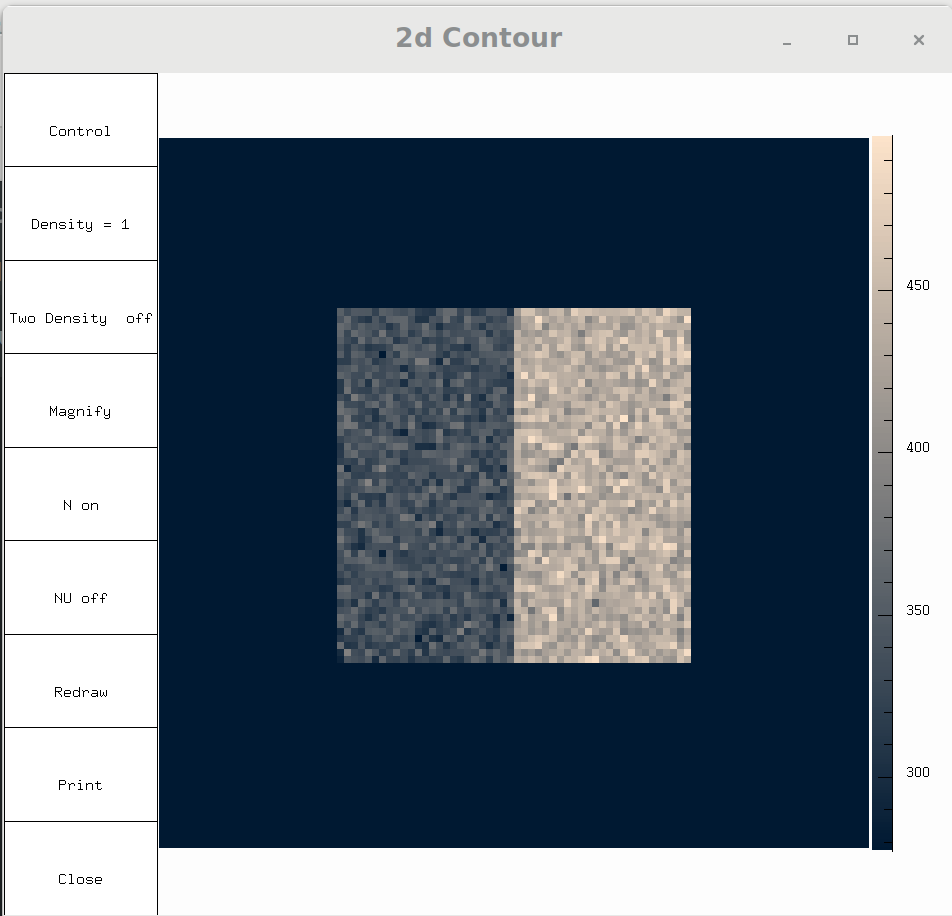
\includegraphics[scale=0.2]{A1p1}
\caption{}
\end{figure}
<text>
\end{frame}

\begin{frame}
\frametitle{Results}
\begin{figure}
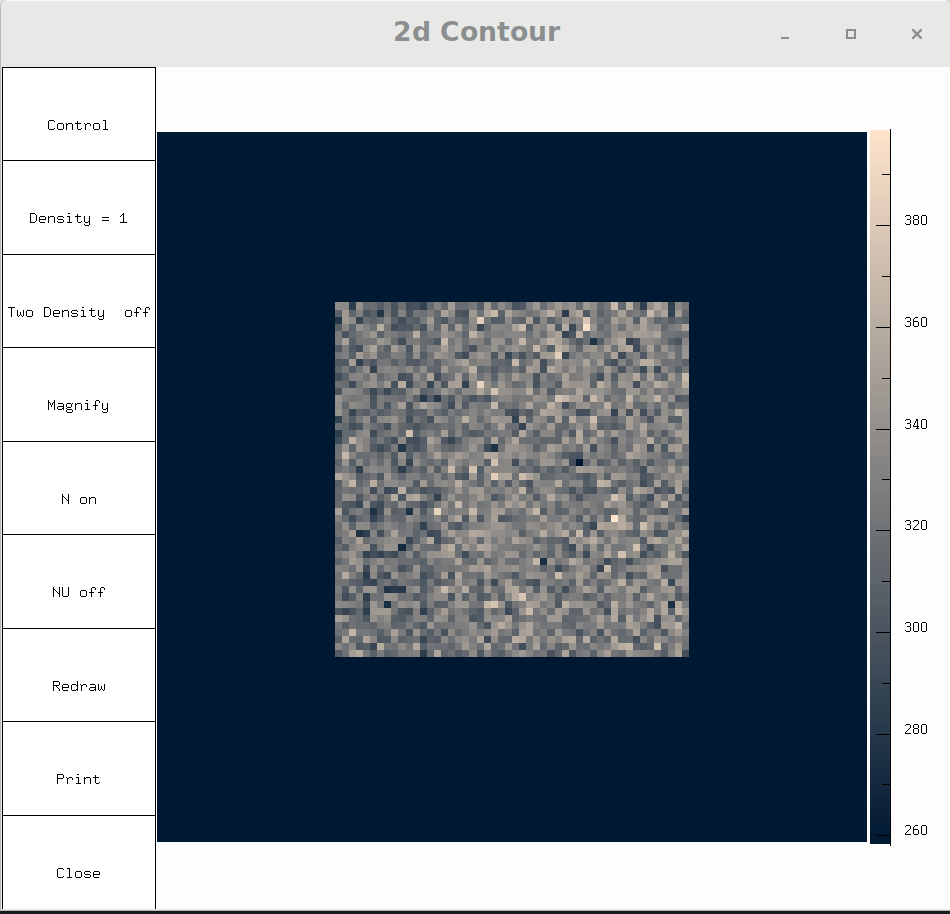
\includegraphics[scale=0.2]{A1p3}
\caption{}
\end{figure}
<text>
\end{frame}

\begin{frame}
\frametitle{Results}
\begin{figure}
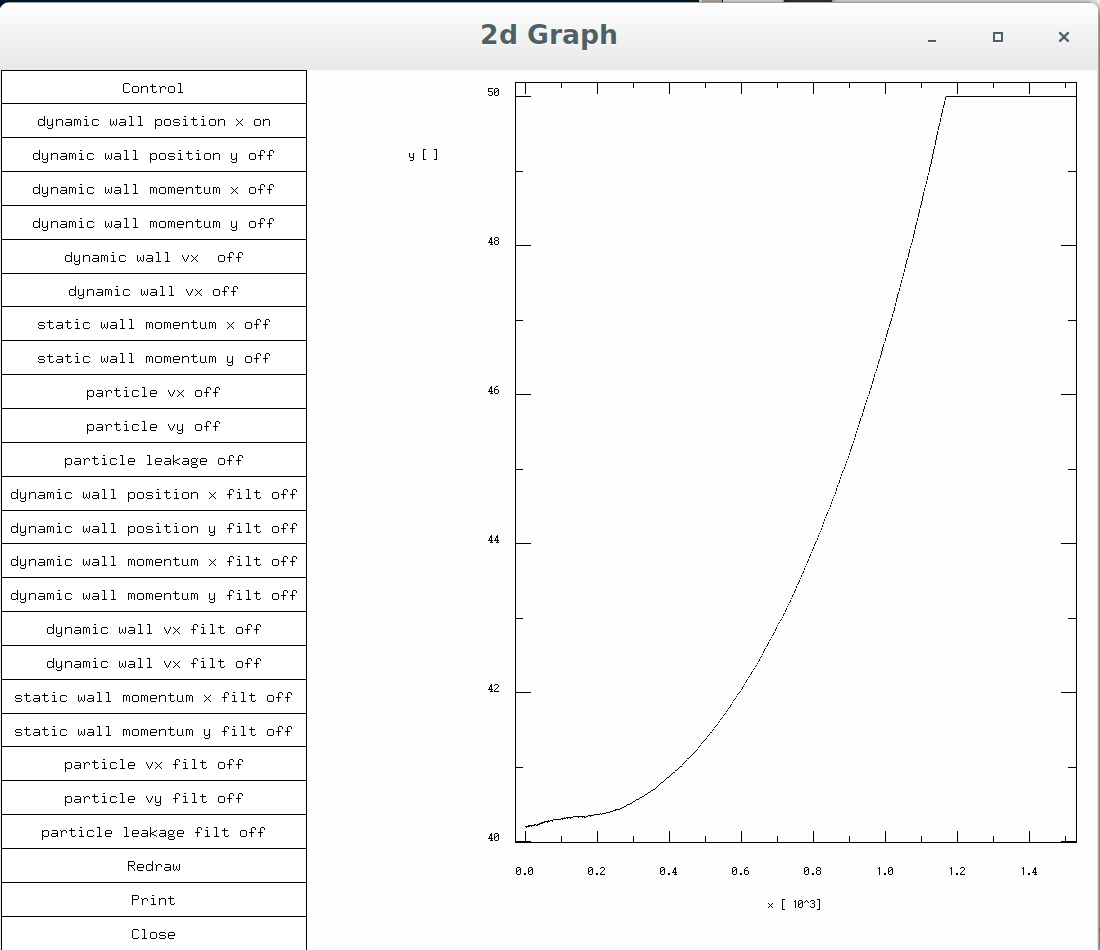
\includegraphics[scale=0.2]{A1p4}
\caption{}
\end{figure}
<text>
\end{frame}

\begin{frame}
\frametitle{Results}
\begin{figure}
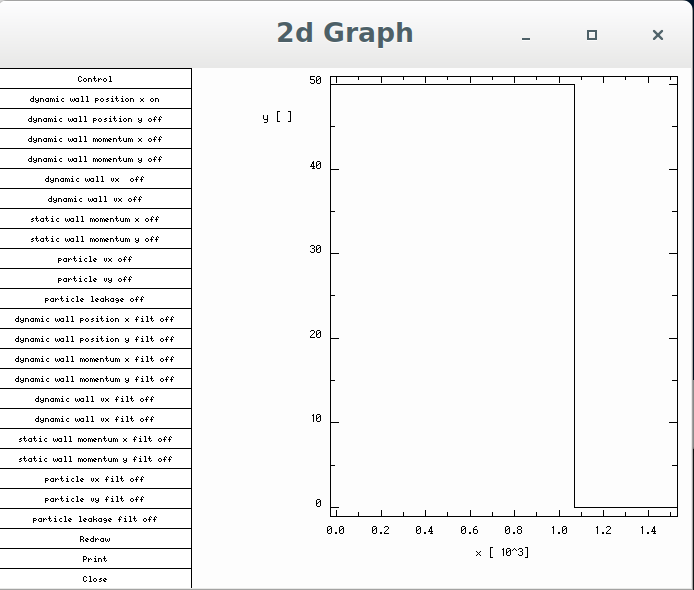
\includegraphics[scale=0.2]{A1p2}
\caption{}
\end{figure}
<text>
\end{frame}

\begin{frame}
\frametitle{Results}
\begin{figure}
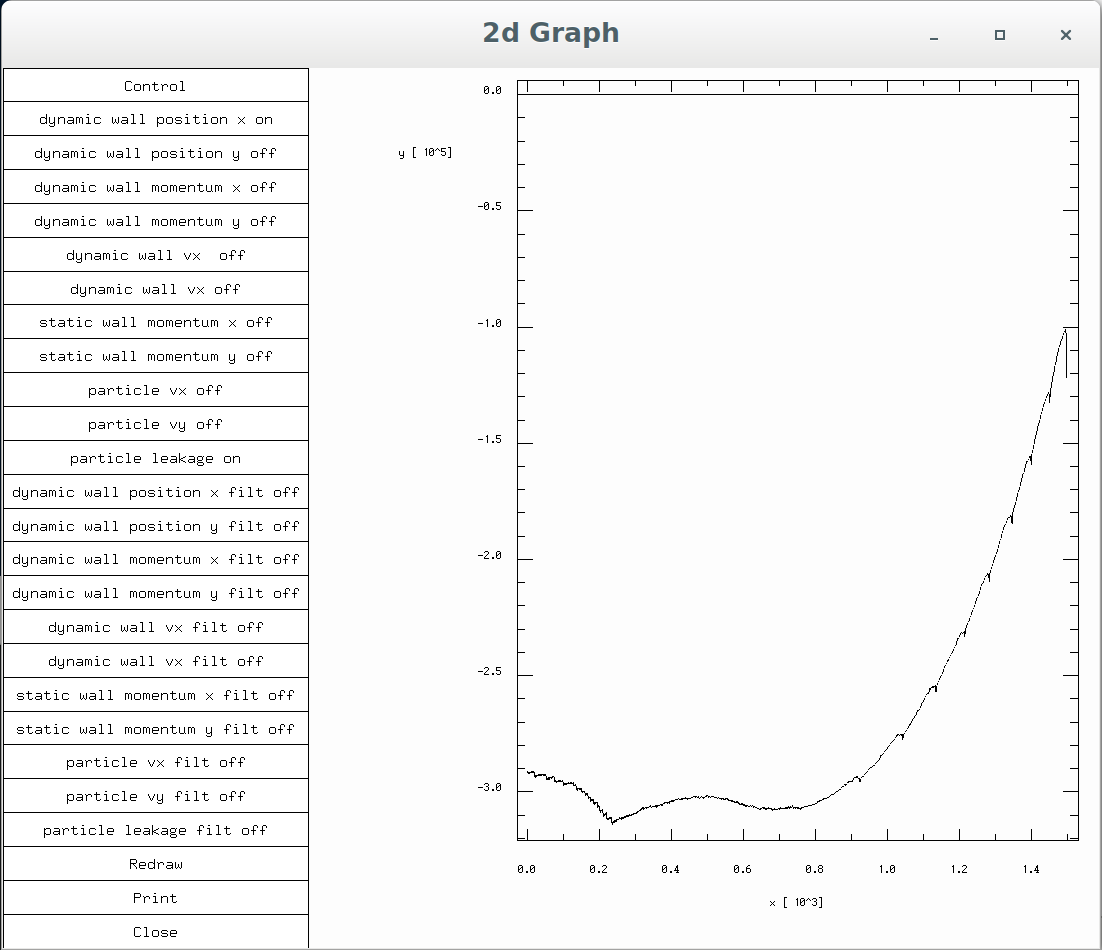
\includegraphics[scale=0.2]{A1p5}
\caption{}
\end{figure}
<text>
\end{frame}


\begin{frame}{Method 2}
In more detail, the probability that $$ pr * \textrm{particle density}$$ number of particles will be moved is $$pr = \frac{\textrm{Wall Vx}}{1-(\textrm{real(Wall x) - int(Wall x)})}$$.
\end{frame}


\begin{frame}[fragile]
\begin{lstlisting}
int tmp = n[x_v_b][y_v_b][v];
int iwp = dynamic_wall_position_x;//integer wall position
int flow = 0;//particles to be moved
double pr = dynamic_wall_vx/(1-(dynamic_wall_position_x - iwp));
if(rand()%1000 <= 1000*pr){
	flow = pr*n[x_b][y_b][v];
	n[x_b+1][y_b][v] +=flow;
	n[x_b][y_b][v] -=flow;}
			
n[x_v_b][y_v_b][v] = n[x_b][y_b][8-v];
n[x_b][y_b][8-v] = tmp;// + flow;	

\end{lstlisting}
\end{frame}

\subsection{Approach 2}
\begin{frame}
\frametitle{Results}
\begin{figure}
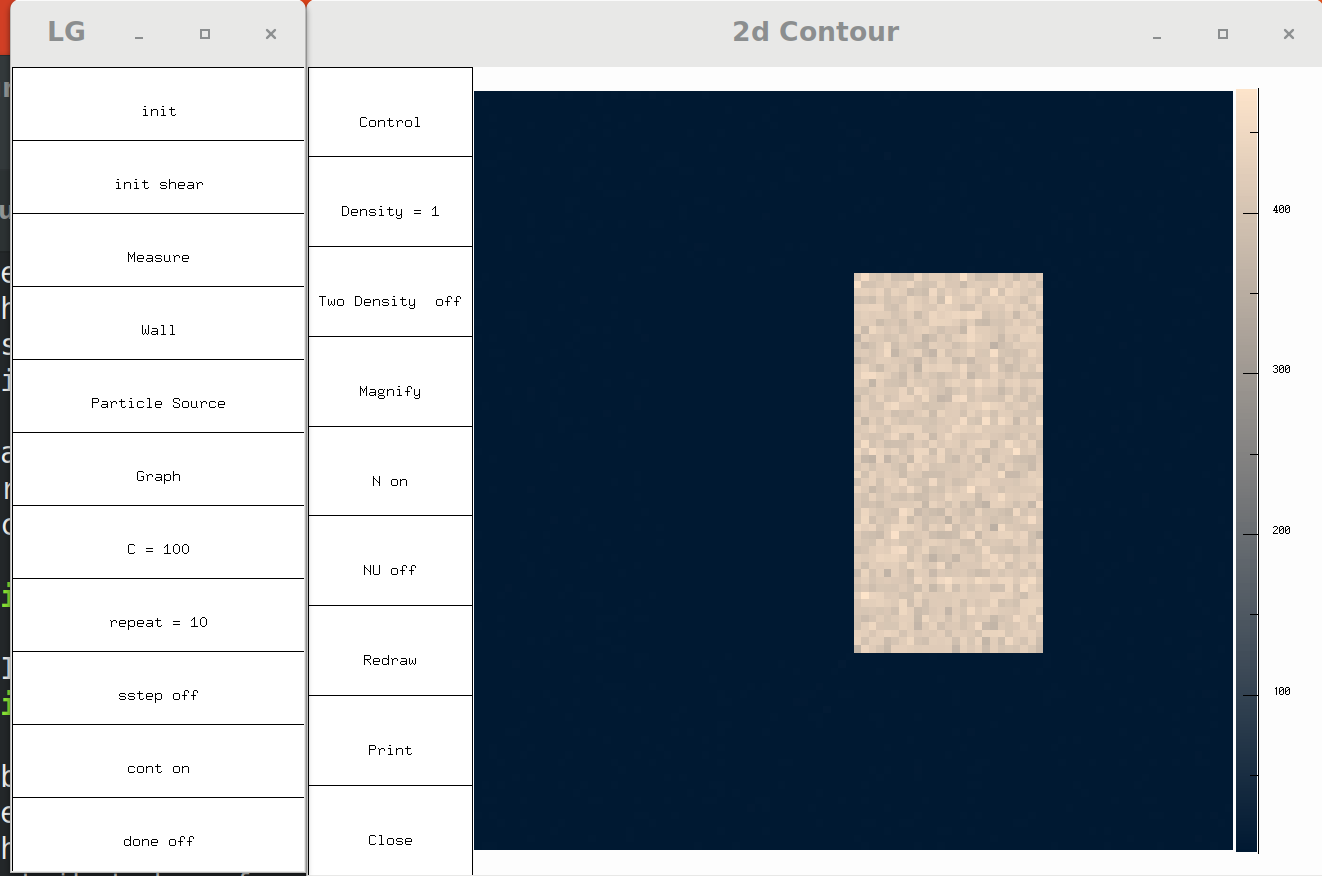
\includegraphics[scale=0.2]{A11p2}
\caption{}
\end{figure}
<text>
\end{frame}

\begin{frame}
\frametitle{Results}
\begin{figure}
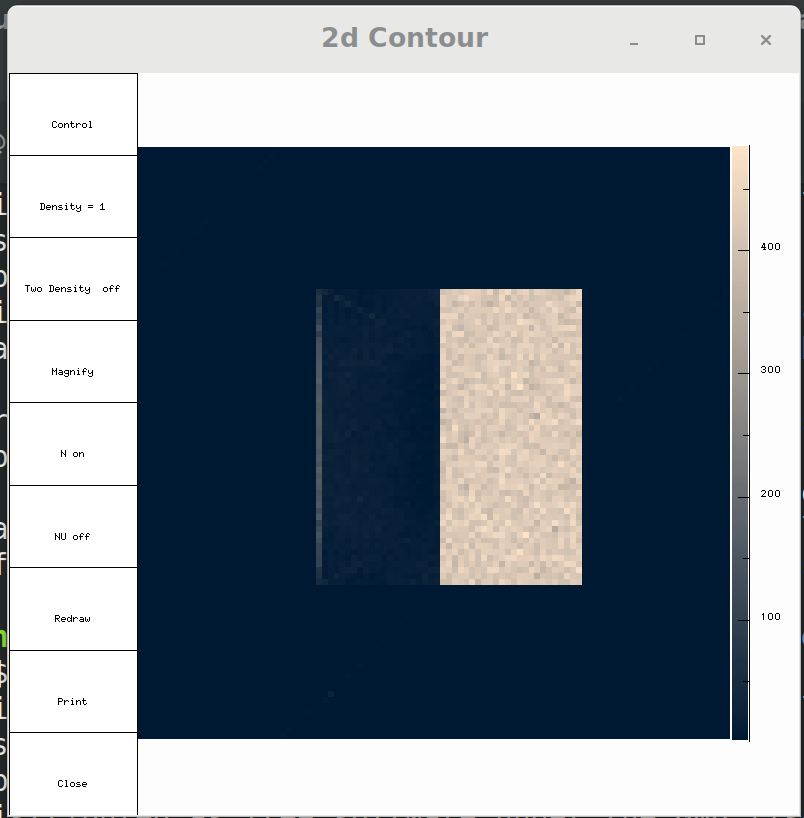
\includegraphics[scale=0.2]{A11p5}
\caption{}
\end{figure}
<text>
\end{frame}

\begin{frame}
\frametitle{Results}
\begin{figure}
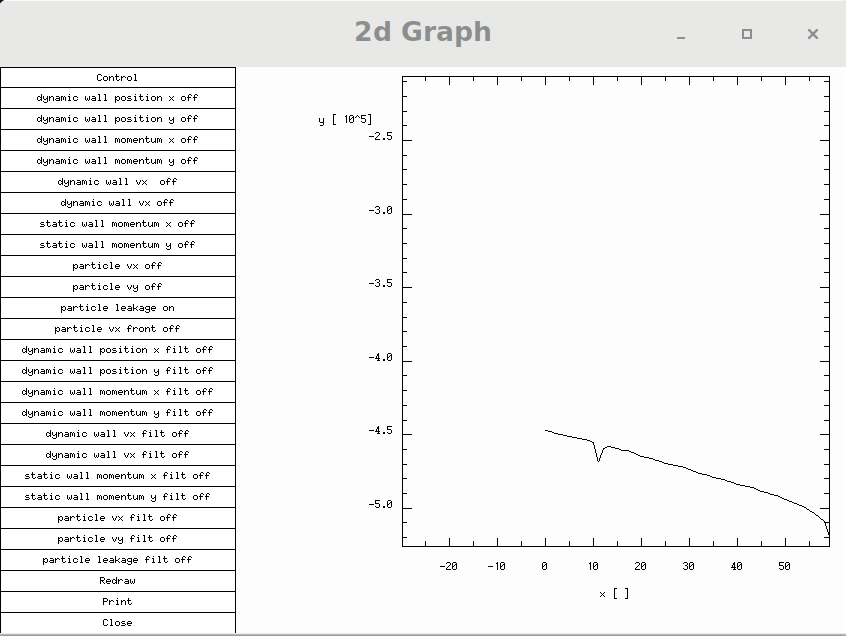
\includegraphics[scale=0.2]{A11p3}
\caption{}
\end{figure}
<text>
\end{frame}

\begin{frame}
\frametitle{Results}
\begin{figure}
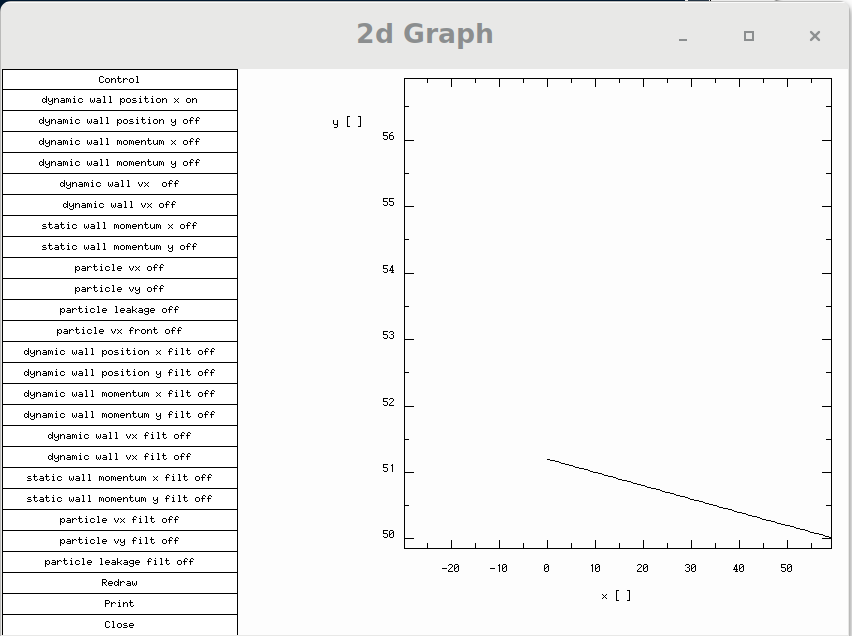
\includegraphics[scale=0.2]{A11p4}
\caption{}
\end{figure}
<text>
\end{frame}

\begin{frame}{Method 3}
\begin{equation}
\frac{\partial \rho}{\partial t} + \frac{\partial(\rho u_{i})}{\partial x_{i}} = \nabla(\rho) + \upsilon *\nabla(\nabla(U)+(\nabla(U)T))
\end{equation}

The partial for $\rho$ and $\rho u_{i}$ can be set to zero.
This gives us:

\begin{equation}
0 = \nabla(\rho) + \upsilon *\nabla(\nabla(U)+(\nabla(U)T))
\end{equation}


$$ \nabla(\rho) = F$$ 

\begin{equation}
0 = F + \upsilon *\nabla(\nabla(U_x))
\end{equation}

Solving the differential equation for $$U_x$$ (mean velocity) above gives us:

\begin{equation}
U_x =\frac{F}{2*\upsilon}*(x(x-L)) \textrm{Where L is the length of the tube in Lattice sites.}
\end{equation}

For C high enough
\begin{equation}
\upsilon = \frac{1}{6}
\end{equation}

\begin{equation}
U_x =F*\frac{6}{2}*(x(x-L)) \textrm{Where L is the length of the tube in Lattice sites.}
\end{equation}

The expected number of particles being moved by a set force is related to the equation below.  
\begin{equation}
<\textrm{particles moved}> = force*\rho
\end{equation}
\end{frame}


\begin{frame}[fragile]
\begin{lstlisting}
void moveParticles(){
for(int x = 0;x<xdim;x++){
 for(int y = 0;y<ydim;y++){
	 int flip_parts = particle_flip_w*
	 ((double)rand()/RAND_MAX)*n[x][y][5];
	 n[x][y][3] += flip_parts;
	 n[x][y][5] -= flip_parts;
	 flip_parts = particle_flip_w*
	 ((double)rand()/(double)RAND_MAX)*n[x][y][8];
	 n[x][y][6] += flip_parts;
	 n[x][y][8] -= flip_parts;
	 flip_parts = particle_flip_w*
	 ((double)rand()/(double)RAND_MAX)*n[x][y][2];
	 n[x][y][0] += flip_parts;
	 n[x][y][2] -= flip_parts;
	}
 }
}
\end{lstlisting}
\end{frame}

\subsection{Approach 3}

\begin{frame}
\frametitle{Results}
\begin{figure}
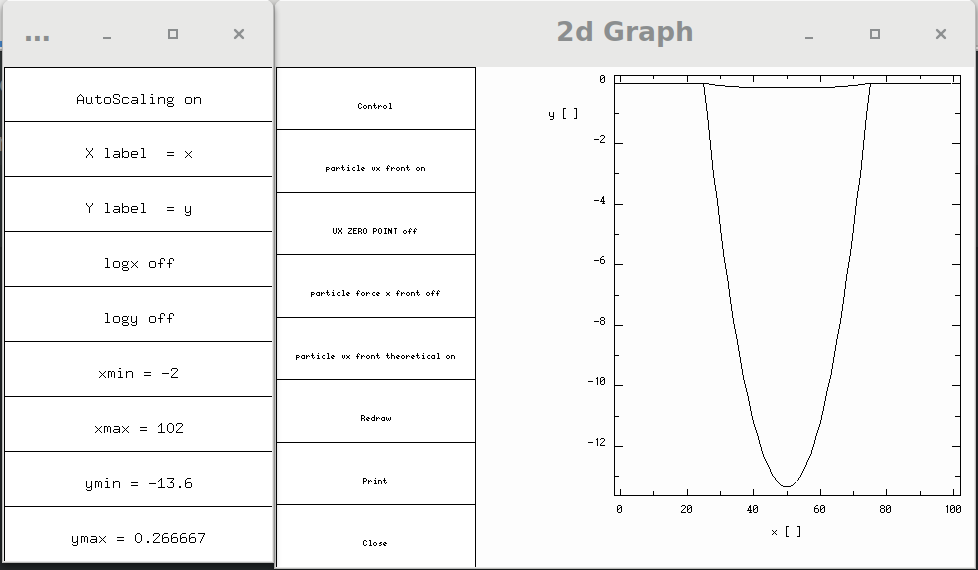
\includegraphics[scale=0.2]{A3p0}
\caption{}
\end{figure}
<text>
\end{frame}

\begin{frame}
\frametitle{Results}
\begin{figure}
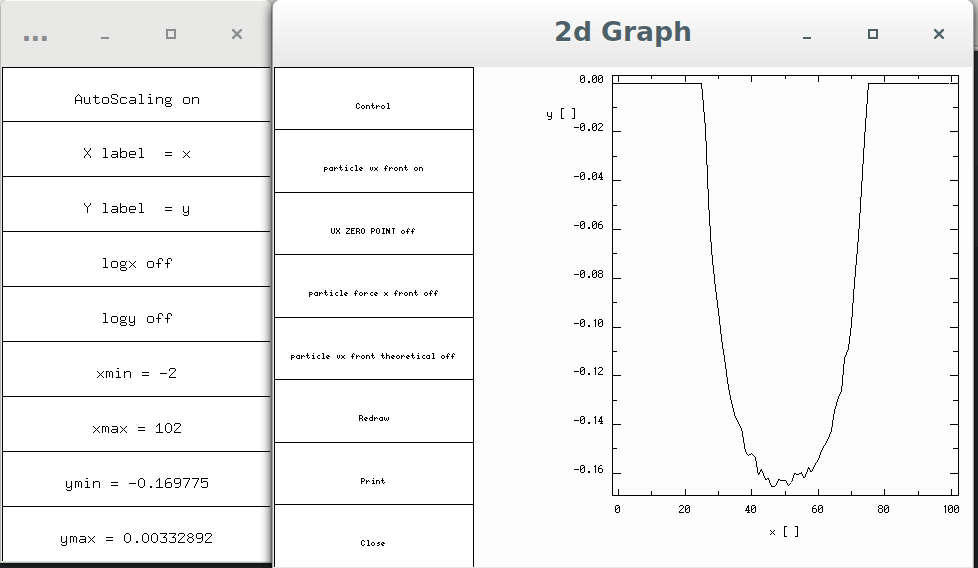
\includegraphics[scale=0.2]{A2p3}
\caption{}
\end{figure}
<text>
\end{frame}

\begin{frame}
\frametitle{Results}
\begin{figure}
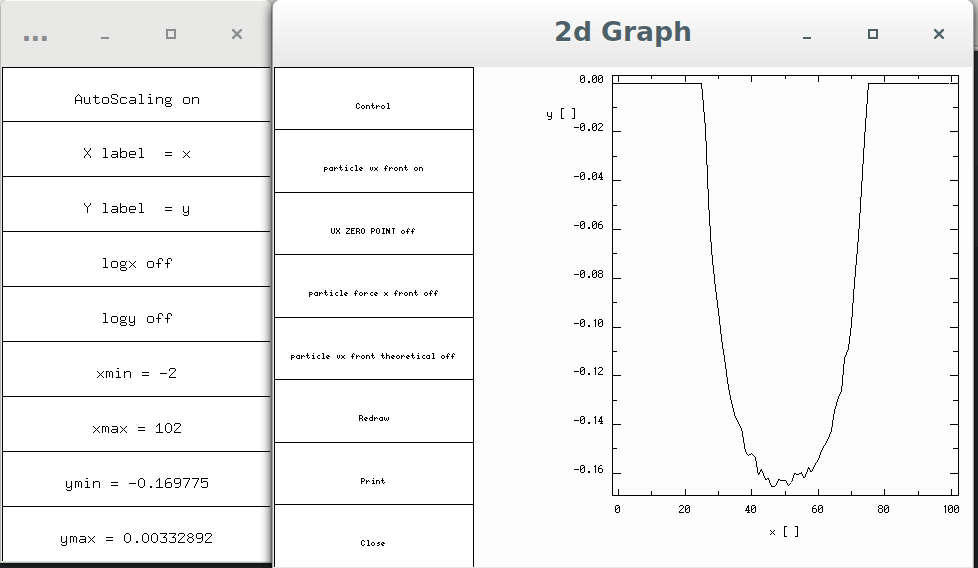
\includegraphics[scale=0.2]{A2p3}
\caption{}
\end{figure}
<text>
\end{frame}
\section{Conclusion}
\begin{frame}{Conclusions and Final thoughts}

\begin{itemize}
  \item Significant leakage for most walls
  \item Partially working
  \item Problem depth and complexity
  \item Approach 3 Issue might be solvable   
\end{itemize}

\vskip 1cm

\end{frame}
\end{document}
